%!mode::"TeX:UTF-8"
\documentclass{ctexart}
\usepackage{amsmath}
\usepackage{amssymb}
\usepackage{xltxtra}
\usepackage{mflogo,texnames}
\usepackage{graphicx}
\usepackage{listings}
\usepackage{listing}
\usepackage{xcolor}
\usepackage{xcolor}
\usepackage{enumerate}
\usepackage[colorlinks,linkcolor=blue]{hyperref}
\usepackage{cite}
\usepackage{color}
\usepackage{caption}
\usepackage{subfigure}
\usepackage[top=2.54cm,bottom=2.54cm,left=3.18cm,right=3.18cm]{geometry}
\author{右武卫大将军}
\title{视觉增强学习}
\begin{document}
    \maketitle
    \section{摘要}
        我们提出一种基于语义层对照片图像进行分解合成的方法。在给定语义标签映射的基础上,该方法可以给出一个符合输入层要求的分解图片。因此该方法实质上就是可以接受关于一个场景的二维语义描述,而生成相应图片的工具。不同于最近的其他一些方法,我们的这个方法并不依赖于对抗性训练。我们要说明的是,图片可以通过一个简单的具有恰当结构的前向网络从语义层进行分解,并且训练的过程是针对特定目标的端对端的训练。这种方法可以无缝测量很好的解析度;我们通过分解2M 分辨率的图片来说明这一问题,这一分辨率是训练图片的最大分辨率。在不同的室内或者室外场景下额外感知试验表明这一方法在图片分解上比其他方法具有更强的可用性。
    \section{介绍}
        如图1 中的语义层画面,一个经验丰富画家可以基于这一画面绘制出逼真的图像。那么能不能训练一个机器模型来实现这一功能呢?即给定一个画面的基本构造描述,然后智能系统就可以绘制出相应的伪造照片。这一问题是计算机图像学和人工智能的中心问题之一。首先,在计算机仿真图像的角度下谈这个问题。可以从语义层合成照片级图片的系统实际上扮演了一种传递机器,这个机器绕过复杂的三维几何,表面的反光情况以及空间中的光影。直接的合成方法可能还不会直接取代现代的透视机制,但是说明这是现存计算机图像学的一个有效替代。

        我们第二个目标是将人类心中的画像模拟出来。心理画面在计划和决策中扮演了重要的角色。这种精细度和完成度的心理画像还是有争议的,但是它在人类认知中的角色说明照片级图像合成是人工智能系统发展的基石。

        在本文中,构建了一个基于像素级语义层的照片合成系统。我们的模型是一个卷积神经网络,在成对的照片和对应的语义图片上进行有监督范式的训练。数据来自于语义分割数据集。我们使用这一数据集的目的并不是从图片来获取语义层而是从语义层来合成图片。图片合成的结果如图1 所示。

        我们会说明这种照片级图像可以直接通过训练一个前向卷积网络来最小化回归损失来实现。这不同于之前的通过生成对抗学习来完成,生成对抗学习方法的弊端在于特别不稳定。本文的方法可以将图片调整到分辨率特别高的水平。每一层的处理都会使图片的分辨率翻倍。

    \section{方法}
        \subsection{准备工作}
            考虑一个语义层$L \in {0,1}^{m\times n \times c}$,其中$m\times n$ 是分辨率,而$c$ 是语义类别的个数。在$L$ 中的每一个像素点代表着一个0/1 编码向量来指示它的语义标签。
            \begin{equation}
                \begin{split}
                    L(i,j) \in \{0,1\}^c \\
                    s.t.\ \sum_pL(i,j,p) = 1
                \end{split}
            \end{equation}
            在$c$ 个可能的标签里有一个标签代表空值,即该位置的物体并没有指明。我们的目标是给定一个语义图像$L$,训练一个参数化的映射关系$g$,可以生成与$L$ 相对应的彩色图片$I\in \mathbb{R}^{m\times n \times 3}$。

            在项目过程中,我们试验了大量的网络架构,结果表明,有三种特征会显著影响照片合成工作。我们先来介绍一下这三种特征:
            \begin{enumerate}
                \item \textbf{全局的协调性(Global Coordination)}全局的一致性结构是图片合成工作的必要点。有很多物体存在非局部的结构关系,比如对称性。如果模型在车的左侧构造了一个红灯,那么在车的右侧也应该有一个红灯。这一点上图像合成与文本合成有很大的不同。这一点也能够提升模型的统计稳定性。我们的模型是基于多次分辨率强化的,这种对称性在极低分辨率的情况下就存在了。特征映射在这个过程中不断强化。因此全局结构在较低分辨率上就已经开始相互协调,高分辨率上距离较远的一致性要求,在低分辨率上通常是相邻的。

                \item \textbf{高分辨率(High Resolution)} 为了生成真实的照片,模型必须能够合成高分辨率的图片。低分辨率的图片通常看上去像近视患者的感受,很好的视觉特征也无法展现。不同行业对于高分辨率图像和视频的要求也说明了高分辨率的重要性。我们的模型会逐步的提高合成图片的分辨率,方法是添加一个简单的增强模型。整个的级联强化模型的训练是端对端的。

                \item \textbf{内存(Memory)} 我们认为模型的巨大容量对于合成高分辨率图片具有非常重要的作用。最好的压缩算法为存储一张高分辨率图片也需要很大的空间,事实证明,目前没有办法从一个低容量的存储中还原出高清图片。所以为了支持我们的模型从一个较为简单的语义图片合成各种各样的高分辨率图片,模型的容量就必须要非常大。我们期望模型既可以在训练集上表现良好,也希望它在测试集上表现良好,这就要求模型的容量很大。我们的设计是模块化的,并且模型的容量可以随着硬件的提升而扩展。目前实验中使用的模型有大约105M 个参数,是对GPU 内存的最大利用了,我们观察到模型的容量越大,图片的质量越高。

            \end{enumerate}
        \subsection{结构}
            级联强化网络(Cascaded Refinement Network,CRN)是将强化单元串联起来的模型。每一个单元模型$M^i$ 在给定的分辨率上进行工作。在我们的实现中,第一个单元的分辨率是$4\times 8$ 的,分辨率在两个相邻的单元中(从$M^{i-1}$ 到$M^i$)是翻倍的。记第$i$ 个单元的分辨率为$w_i \times h_i$。

            第一个单元$M^0$,接受语义图层$L$ 作为输入,降采样为$w_0 \times h_0$,进而生成一个特征层$F^0$,分辨率是$w_0 \times h_0$,作为输出。其他的后续单元的构成如下:$M_i$ 接收一个语义图层(降采样至$w_i \times h_i$)和上一单元所输出的特征$F^{i-1}$ (升采样到$w_i \times h_i$)的拼接图块作为输入,然后输出相应的特征$F^i$。 我们将输出图块$F^i$ 的特征层数记为$d_i$。

            \textbf{降采样}:就是缩小图像,使图像的大小满足神经网络的输入尺寸要求。降采样的原理是,对于一个图像的尺寸为$M\times N$,选取$M$ 和$N$ 的公约数$S$,在该图像$S\times S$ 的方形像素窗口中合并为一个像素点,值为
            $$
                v^* = \sum_{i \in S^2} v_i/S^2
            $$
            如此降采样之后的图像尺寸为$M/S\times N/S$。

            \textbf{升采样}:就是放大图像,使图像满足神经网络的输入尺寸要求。升采样的原理是在图片的像素点之间进行插值来放大图片。最常用的方法是双线性插值,具体方法如下图:
            \begin{figure}[h]
                \centering
                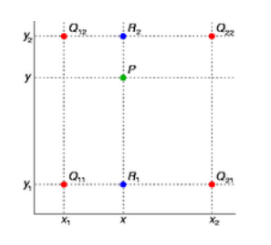
\includegraphics[width=0.6\textwidth]{1}
                \caption{双线性插值的原理}
                \label{f_1}
            \end{figure}

            每一个单元$M^i$ 由三个不同的组件构成:输入层,隐藏层,输出层。如图3 所示。输入层的维度为$w_i \times h_i \times (d_{i-1} + c)$,接受的是降采样之后的语义图层(有$c$ 个通道)和一个双线性升采样的特征层$F^{i-1}$ ($d_{i-1}$ 个通道)。这里没有使用上卷积方法的原因是上卷积通常会导入较多的主观误差。中间层和输出层的维度都是$w_i\times h_i \times d_i$。 每一层后面都跟着一个$3\times 3$ 的卷积层,层标准化和LReLU 激活映射。

            最后一个单元$M^{\bar{\iota}}$ 的输出$F^{\bar{\iota}}$ 不进行标准化和非线性激活映射。取而代之的是,使用一个线性投影($1\times 1$ 卷积)作用在$F^{\bar{\iota}}$ (尺寸为$w_{\bar{\iota}} \times h_{\bar{\iota}} \times d_{\bar{\iota}}$)输出一个彩色图片(尺寸为$w_{\bar{\iota}}\times h_{\bar{\iota}} \times 3$)。强化单元的级联个数取决于最终输出的分辨率。在我们在实验中,级联的个数为9 个,将分辨率从$4\times 8$ 增加到$1024\times 2048$,而每一层的通道数为:0 到4 单元为1024 个通道,5,6 单元为512 个通道,7 单元为128 个通道,8 单元为32 个通道。

        \subsection{训练}
            CRN 模型在语义分割数据集$\mathcal{D}=\{(I,L)\}$ 使用有监督学习范式进行训练。语义分割层$L$ 作为输入,相对应的彩色图片$I$ 为输出。也就是说这一工作可以被认为是“逆语义切割”。不过它是一个一对多的非严格的逆问题。所以我们把原始图片$I$ 称为“参考图片”,而不是“实际图像”,因为可能不同配色的图片也可以产生同样的语义分割图片。

            由于这一问题是非严格限定的,所以选择恰当的损失函数非常重要。简单地对比合成图片和原始图片在像素点上的差异会对很多逼真的合同结果产生很大的惩罚。比如,合成图片上是一个白色汽车而原始图片上是一个黑色汽车会产生很大的“误差”。所以我们采用Gatys 等介绍的内容表示损失,也参考了诸多参考文献中的“特征匹配损失”。基本思想是引入一个效果较好的图像识别网络,利用该网络在合成图片和参考图片上所抽取的特征的相似程度作为损失。

            记$\Phi$ 是一个已经训练好的视觉感知网络(本文使用的是VGG-19)。随着卷积层数的增加,特征抽取的抽象级别逐步提高,从线条和颜色逐步提高到物体和类别。既需要合成图片的模型能够在低级别的层次上匹配也需要在高层次上匹配,这样保证了合成图片在细节和全局布局上都具有和参考图片相似的特征。

            记$\{\Phi_l\}$ 是模型$\Phi$ 中的一组网络层,比如$\Phi_0$ 代表输入层。每一层有一个三维的张量。对于训练组$(I,L)\in \mathcal{D}$,相应的损失函数为
            \begin{equation}
                \mathcal{L}_{I,L}(\theta) = \sum_l \lambda_l \|\Phi_l(I) - \Phi_l(g(L;\theta))\|_1
            \end{equation}
            其中$g$ 是图片合成模型,而$\theta$ 是模型中的参数。而相应的超参数$\lambda_l$ 平衡了每一层特征在总体损失中的权重。

            对于$\Phi_l(l \le 1)$,我们选用了VGG-19 网络中的“$conv1-2$”,“$conv2-2$”,“$conv3-2$”,“$conv4-2$”,“$conv5-2$”。其中超参数组$\{\lambda_l\}$ 是自动设置的。他们的初始值是每一层中元素数量的倒数。在进行100 次循环训练之后,$\{\lambda_l\}$ 被重新设定为可以标准化每一项$\|\Phi_l(I) - \Phi_l(g(L;\theta))\|_1$ 损失的合适的值。
        \subsection{合成图片的多样性}
            网络架构和训练过程在上面两节已经介绍了。到这一步,模型已经能够产生不错的结果了。但是,因为给定一个语义图层对应着很多图片,所以如果模型能够给出一组合成图片也是有意义的。我们会通过将损失函数修改为能够鼓励多样化输出的损失函数的方式来使模型可以输出多样化的图片。

            具体来说,我们把输出通道由3 个改成$3k$ 个,其中$k$ 是希望获得到的图片数量。每一组连续的三个通道构成一张图片。接下来考虑损失的问题。如果上面介绍的损失函数应用在每一组(3个通道)上,那么$k$ 个合成图片都是一样的。第一个修正点是将$k$ 张合成图片在一起考虑,进而定义一个全局最优的合成图片。记$g_u(L;\theta)$ 是合成图片集合中的第$u^{th}$ 张图片。修正损失函数的第一个版本是基于为多结果学习而设计的滞后损失函数:
            \begin{equation}
                \min\limits_u \sum_l \lambda_l\|\Phi_l(I) - \Phi_l(g_u(L;\theta))\|_1
            \end{equation}
            通过只考虑最优的那张合成图片,该损失函数鼓励模型充分的探索特征空间。这一损失函数在结构上类似于$k$ 均值聚类,只考虑距离该点最近的那个质心所带来的损失,这样,其他质心可以充分探索特征空间。

            我们进一步强化这一思想,构建一个考虑多达$k^c$ 张图片的虚拟图片集合的损失函数,其中$c$ 是语义图层类别的个数。具体来说,对于每一个语义类别$p$,记$L_p$ 为输入语义图层中相应的通道$L(.,. ,p)$,我们定义一个更有力的多样化损失函数:
            \begin{equation}
                \sum_{p=1}^c \min\limits_u \sum_l \lambda_l \sum_j \|L_p^l \odot (\Phi_l^j(I) - \Phi_l^j(g_u(L;\theta)))\|_1
            \end{equation}
            其中$\Phi_l^j$ 是$\Phi_l$ 中的第$j^{th}$ 个特征通道,$L_p^l$ 是$L_p$ 降采样到$\Phi_l$ 的尺寸上的结果,而$\odot$ 是Hadamard 矩阵积,即对应元素相乘。实际上该损失通过为每一个语义类别选取最优的合成内容来构建虚拟图片,然后基于图片集合来评估损失。


\end{document}
